\documentclass[xcolor=pdftex,dvipsnames,table,mathserif,aspectratio=169]{beamer}
\usetheme{default}
\usetheme{metropolis}
\usepackage{minted}
\usepackage{mathtools}
\setbeamersize{text margin left=.3in,text margin right=.3in} 

\DeclarePairedDelimiter\abs{\lvert}{\rvert}%
\DeclarePairedDelimiter\norm{\lVert}{\rVert}%

\usepackage[english]{babel}
\usepackage{pgf,pgfarrows,pgfnodes,pgfautomata,pgfheaps}
\usepackage{amsmath,amssymb,setspace,centernot}
\usepackage[latin1]{inputenc}
\usepackage{pgf,tikz}
\usepackage[T1]{fontenc}
\usepackage{relsize}
\usepackage{pdfpages}
\usepackage[absolute,overlay]{textpos} 


\newenvironment{reference}[2]{% 
  \begin{textblock*}{\textwidth}(#1,#2) 
      \footnotesize\it\bgroup\color{red!50!black}}{\egroup\end{textblock*}} 

\DeclareMathSizes{10}{10}{6}{6} 

\begin{document}
\title{Multinomial Discrete Choice: Beyond Logit}
\author{Chris Conlon}
\institute{Applied Econometrics II}
\date{\today}

\frame{\titlepage}

\begin{frame}
\frametitle{Multinomial Logit: IIA}
The multinomial logit is frequently criticized for producing unrealistic substitution patterns
\begin{itemize}
\item Suppose we got rid of a product $k$ then $s_j^{(1)} = s_j^{(0)} \frac{1}{1- s_k}$.
\item Substitution is just proportional to your pre-existing shares $s_j$
\item No concept of ``closeness'' of competition!
\end{itemize}
\end{frame}

\begin{frame}
\frametitle{Can we do better?}
Multinomial Probit?
\begin{itemize}
\item The probit has $\varepsilon_i \sim N(0,\Sigma)$.
\item If $\Sigma$ is unrestricted, then this can produce relatively flexible substitution patterns.
\item Flexible is relative: still have normal tails, only pairwise correlations, etc.
\item It might be that $\rho_{12}$ is large if $1,2$ are similar products.
\item Much more flexible than Logit
\end{itemize}
Downside
\begin{itemize}
\item $\Sigma$ has potentially $J^2$ parameters (that is a lot)!
\item Maybe $J * (J-1)/2$ under symmetry. (still a lot).
\item Each time we want to compute $s_j(\theta)$ we have to simulate an integral of dimension $J$.
\item I wouldn't do this for $J \geq 5$.
\end{itemize}
\end{frame}

\begin{frame}
\frametitle{Relaxing IIA}
Let's make $\varepsilon_{ij}$ more flexible than IID. Hopefully still have our integrals work out.
\begin{eqnarray*}
u_{ij} =   x_{ij} \beta  + \varepsilon_{ij}
\end{eqnarray*}
\begin{itemize}
\item One approach is to allow for a block structure on $\varepsilon_{ij}$ (and consequently on the elasticities).
\item We assign products into groups $g$ and add a group specific error term
\begin{eqnarray*}
u_{ij} =   x_{ij} \beta  + \eta_{g} + \varepsilon_{ij}
\end{eqnarray*}
\item The trick putting a distribution on $\eta_g + \varepsilon_{ij}$ so that the integrals still work out.
\item Do not try this at home: it turns out the required distribution is known as \alert{GEV} and the resulting model is known as the \alert{nested logit}.
\end{itemize}
\end{frame}

\begin{frame}{Nested Logit}
A traditional (and simple) relaxation of the IIA property is the Nested Logit. This model is often presented as two sequential decisions.
\begin{itemize}
\item First consumers choose a category (following an IIA logit).
\item Within a category consumers make a second decision (following the IIA logit).
\item This leads to a situation where while choices within the same nest follow the IIA property (do not depend on attributes of other alternatives) choices among different nests do not!
\end{itemize}
\end{frame}

\begin{frame}{Alternative Interpretation}
\begin{figure}[htbp]
\begin{center}
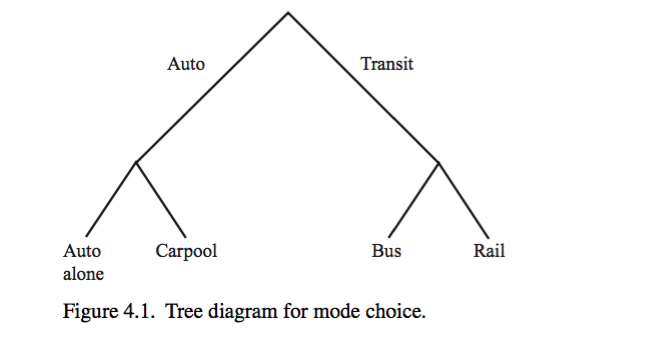
\includegraphics[width=5in]{resources/nesting.png}
\end{center}
\end{figure}
\end{frame}

\begin{frame}{Nested Logit}
Utility looks basically the same as before:
\begin{eqnarray*}
U_{ij} = V_{ij} + \underbrace{\eta_{ig} + \widetilde{\varepsilon_{ij}}}_{\varepsilon_{ij}(\lambda_g)}
\end{eqnarray*}
\begin{itemize}
\item We add a new term that depends on the group $g$ but not the product $j$ and think about it as varying unobservably over individuals $i$ just like $\varepsilon_{ij}$.
\item Now $\varepsilon_i \sim F(\varepsilon)$ where $F(\varepsilon) = \exp[-\sum_{g=G}^G \left(\sum_{j \in J_g} \exp[-\varepsilon_{ij}/\lambda_g]\right)^{\lambda_g}$. This is no longer Type I EV but GEV.
\item The key is the addition of the $\lambda_g$ parameters which govern (roughly) the within group correlation.
\item This distribution is a bit cooked up to get a closed form result, but for $\lambda_g \in [0,1]$ for all $g$ it is consistent with random utility maximization.
\end{itemize}
\end{frame}

\begin{frame}{Nested Logit}
\small
The nested logit choice probabilities are:
\begin{eqnarray*}
s_{ij} = \frac{ e^{V_{ij}/\lambda_g} \left(\sum_{k \in J_g} e^{V_{ik}/\lambda_g} \right)^{\lambda_g -1}}{\sum_{h=1}^G \left(\sum_{k \in J_h} e^{V_{ik}/\lambda_h} \right)^{\lambda_h}}
\end{eqnarray*}
Within the same group $g$ we have IIA and proportional substitution 
\begin{eqnarray*}
\frac{s_{ij}}{s_{ik}} = \frac{ e^{V_{ij}/\lambda_g}}{ e^{V_{ik}/\lambda_g}}
\end{eqnarray*}

But for different groups we do not:
\begin{eqnarray*}
s_{ij} = \frac{ e^{V_{ij}/\lambda_g} \left(\sum_{k \in J_g} e^{V_{ik}/\lambda_g} \right)^{\lambda_g -1}}{ e^{V_{ik}/\lambda_h} \left(\sum_{k \in J_h} e^{V_{ik}/\lambda_h} \right)^{\lambda_h -1}}
\end{eqnarray*}
\end{frame}


\begin{frame}{Nested Logit}
We can take the probabilities and re-write them slightly with the substitution that 
$\log \left(\sum_{k \in J_g} e^{V_{ik}} \right)\equiv IV_{ig}$:
\begin{eqnarray*}
s_{ij} &=& \frac{ e^{V_{ij}/\lambda_g}}{ \left(\sum_{k \in J_g} e^{V_{ik}/\lambda_g} \right)}
\cdot
\frac{ \left(\sum_{k \in J_g} e^{V_{ik}/\lambda_g} \right)^{\lambda_g}}{\sum_{h=1}^G \left(\sum_{k \in J_h} e^{V_{ik}/\lambda_h} \right)^{\lambda_h}} \\
&=& \underbrace{\frac{ e^{V_{ij}/\lambda_g}}{ \left(\sum_{k \in J_g} e^{V_{ik}/\lambda_g} \right)}}_{s_{i j | g}}
\cdot
\underbrace{\frac{e^{\lambda_g IV_{ig}}}{\sum_{h=1}^{G} e^{\lambda_h IV_{ih}} }}_{s_{ig}}
\end{eqnarray*}
This is the decomposition into two logits that leads to the ``sequential logit'' story.
\end{frame}

\begin{frame}{Nested Logit : Notes}
\begin{itemize}
\item $\lambda_g=1$ is the simple logit case (IIA)
\item $\lambda_g \rightarrow 0$ implies that all consumers stay within the nest.
\item $\lambda < 0$ or $\lambda > 1$ can happen and usually means something is wrong. These models are not generally consistent with RUM. (If you report one in your paper I will reject it).
\item $\lambda$ is often interpreted as a correlation parameter and this is almost true but not exactly!
\item There are other extensions: overlapping nests, or three level nested logit. 
\item In general the hard part is understanding what the appropriate nesting structure is ex ante. Maybe for some problems this is obvious but for many not.
\end{itemize}
\end{frame}

%\begin{frame}{Nested Logit : Interpretation}
%\begin{itemize}
%\item It is convenient to think about the ``sequential choice'' version of the nested logit.
%\item In practice it is more accurate to think about the structure it imposes on the correlation of $\varepsilon_i$. 
%\item We specify a blocked structure (one block for each nest) and estimate a within vs. across nest correlation parameter.
%\end{itemize}
%\end{frame}


\begin{frame}
\frametitle{Nested Logit}
In practice we end up with the following:
\begin{eqnarray*}
s_{ij} = s_{ij|g}(\theta) s_{ig}(\theta)
\end{eqnarray*}
\vspace{-0.5cm}
\begin{itemize}
\item Because the nested logit can be written as the within group share $s_{ij|g}$ and the share of the group $s_{ig}$ we often explain this model as \alert{sequential choice}
\item First you pick a category, then you pick a product within a category.
\item This is a sometimes helpful (sometimes unhelpful) way to think about this.
\item We can also think about this imposing a block structure on the covariance matrix of $\varepsilon_i$
\item You need to assign products to categories \alert{before you estimate} and you can't make mistakes!
\end{itemize}
\end{frame}

\begin{frame}
\frametitle{Nested Logit}
How does it actually look?
\begin{eqnarray*}
 IV_{ig}(\theta) &=& \log \left(\sum_{k \in G} \exp [x_k \beta/(1-\lambda_g)] \right) = E_{\varepsilon}[\max_{j \in G} u_{ij}]\\
 s_{ij|g}(\theta) &=& \frac{\exp [x_j \beta/(1-\lambda_g)]}{\sum_{k \in G} \exp [x_k \beta/(1-\lambda_g)]} \\
 s_{ig}(\theta) &=& \frac{\exp [IV_{ig}]^{1-\lambda_g}}{\sum_{h} \exp [IV_{ih}]^{1-\lambda_h}} 
\end{eqnarray*}
%\begin{itemize}
%\item When $\lambda_g \rightarrow 0$ we get the IIA logit model (no correlation within nests)
%\item When $\lambda_g \rightarrow 1$ we get no across nest substitution.
%\item When $\lambda_g > 1$ we get something not necessarily consistent with utility maximization!
%\end{itemize}
\end{frame}

\begin{frame}
\frametitle{Nested Logit}
How does it actually look?
\begin{eqnarray*}
\log \left(\frac{s_{ij|g}(\theta)}{s_{ik|g}(\theta)} \right) = (x_j -x_k)\cdot \frac{\beta}{1-\lambda_g}
 \end{eqnarray*}
 \begin{itemize}
\item We are back to having the IIA property but now within the group $G$.
\item We also have IIA across groups $g,h$
\item $\lambda_g$ and $\alpha$ govern the elasticities, which also have a block structure. % expand this later
\item Sometimes people refer to this as the \alert{product of two logits}
\item In the old days people used to estimate by fitting sequential IIA logit models -- this is consistent but inefficient -- you shouldn't do this today!
\item Estimation happens via MLE. This can be tricky because the model is non-convex. It helps to substitute $\tilde{\beta} = \beta/(1-\lambda_g)$
 \end{itemize}
\end{frame}

\begin{frame}
\frametitle{Parametric Identification}

Look at derivatives:
\begin{eqnarray*}
\frac{\partial\, s_{j|g}}{\partial X_j} &=& \beta_1 s_{j|g}(1-s_{j|g}) \\
 \frac{\partial\, s_{g}}{\partial X} &=& (1-\lambda) \beta_1 s_{g}(1-s_{g}) \\
  \frac{\partial\, s_{g}}{\partial J} &=& \frac{1-\lambda}{J} s_{g}(1-s_{g})
\end{eqnarray*}
\begin{itemize}
\item We get $\beta$ by changing $x_j$ within group
\item We get nesting parameter $\lambda$ by varying $X$
\item We don't have any parameters left to explain changing number of products $J$.
\end{itemize}

\end{frame}



\begin{frame}
\frametitle{Nested Logit}
There are more potential generalizations though they are less frequently used:
 \begin{itemize}
\item You can have multiple levels of nesting: first I select a size car (compact, mid-sized, full-sized) then I select a manufacturer, finally a car.
\item You can have potentially overlapping nests: Yogurt brands are one nest, Yogurt flavors are a second nest. This way strawberry competes with strawberry and/or Dannon substitutes for Dannon.
 \end{itemize}
\end{frame}


\begin{frame}
\frametitle{Mixed Logit}
We relax the IIA property by mixing over various logits:
\begin{eqnarray*}
u_{ijt} &=& x_j \beta + \mu_{ij} + \varepsilon_{ij} \\
s_{ij} &=& \int \frac{\exp[x_{j} \beta + \mu_{ij} ]}{1+\sum_k \exp[x_{k} \beta + \mu_{ik} ]} f(\boldsymbol{\mu_i} | \theta)
\end{eqnarray*}
 \begin{itemize}
 \item Each individual draws a vector $\boldsymbol{\mu_i}$ of $\mu_{ij}$ (separately from $\varepsilon$).
 \item Conditional on $\boldsymbol{\mu_i}$ each person follows an IIA logit model.
 \item However we integrate (or mix) over many such individuals giving us a \alert{mixed logit} or \alert{heirarchical model} (if you are a statistician)
 \item In practice these are not that different from linear \alert{random effects models} you have learned about previously.
 \item It helps to think about fixing $\boldsymbol{\mu_i}$ first and then integrating out over $\varepsilon_i$
 \end{itemize}
\end{frame}

\begin{frame}{Mixed/ Random Coefficients Logit}
\small
As an alternative, we could have specified an error components structure on $\varepsilon_i$.
\begin{eqnarray*}
U_{ij} = \beta x_{ij} + \underbrace{\nu_i z_{ij} + \varepsilon_{ij}}_{\tilde{\varepsilon}_{ij}}
\end{eqnarray*}
\begin{itemize}
\item The key is that $\nu_i$ is unobserved and mean zero. But that $x_{ij},z_{ij}$ are observed per usual and $\varepsilon_{ij}$ is IID Type I EV.
\item This allows for a heteroskedastic structure on $\varepsilon_{i}$, but only one which we can project down onto the space of $z$.
\end{itemize}
An alternative is to allow for individuals to have random variation in $\beta_i$:
\begin{eqnarray*}
U_{ij} = \beta_i x_{ij} +  \varepsilon_{ij}
\end{eqnarray*}
Which is the random coefficients formulation (these are the same model).
\end{frame}

%
%\begin{frame}{Mixed/ Random Coefficients Logit}
%For each individual $i$, the resulting choice probability follows a logit:
%\begin{eqnarray*}
%P_{ij} = \int \frac{ e^{V_{ij}(\beta_i)}}{\sum_k e^{V_{ik}(\beta_i)}} f(\beta_i | \theta) \partial \beta
%\end{eqnarray*}
%This structure is quite general:
%\begin{itemize}
%\item The choice probabilities are know a function of unknown parameters $\theta$.
%\item We can allow for there to be two types of $\beta_i$ in the population (high-type, low-type). \alert{latent class model}.
%\item We can allow $\beta_i$ to follow an independent normal distribution for each component of $x_{ij}$ such as $\beta_i = \overline{\beta} + \nu_i \sigma$.
%\item We can allow for correlated normal draws using the Cholesky root of the covariance matrix.
%\item Can allow for non-normal distributions too (lognormal, exponential). Why is normal so easy?
%\end{itemize}
%\end{frame}

\begin{frame}{Mixed/ Random Coefficients Logit}
\begin{itemize}
\item Kinds of heterogeneity
\begin{itemize}
\item We can allow for there to be two types of $\beta_i$ in the population (high-type, low-type). \alert{latent class model}.
\item We can allow $\beta_i$ to follow an independent normal distribution for each component of $x_{ij}$ such as $\beta_i = \overline{\beta} + \nu_i \sigma$.
\item We can allow for correlated normal draws using the Cholesky root of the covariance matrix.
\item Can allow for non-normal distributions too (lognormal, exponential). Why is normal so easy?
\end{itemize}
\item The structure is extremely flexible but at a cost.
\item We generally must perform the integration numerically.
\item High-dimensional numerical integration is difficult. In fact, integration in dimension 8 or higher makes me very nervous.
\item We need to be parsimonious in how many variables have unobservable heterogeneity.
\item Again observed heterogeneity does not make life difficult so the more of that the better!
\end{itemize}
\end{frame}

\begin{frame}
\frametitle{Mixed Logit}
How does it work?
 \begin{itemize}
\item Well we are mixing over individuals who conditional on $\beta_i$ or $\mu_i$ follow logit substitution patterns, however they may differ wildly in their $s_{ij}$ and hence their substitution patterns.
\item For example if we are buying cameras: I may care a lot about price, you may care a lot about megapixels, and someone else may care mostly about zoom.
\item The basic idea is that we need to explain the heteroskedasticity of $Cov(\varepsilon_i, \varepsilon_j)$ what random coefficients do is let us use a basis from our $X$'s.
\item If our $X$'s are able to span the space effectively, then an RC logit model can approximate any arbitrary RUM (McFadden and Train 2002). 
\item Of course if you have 1000 products and two random coefficients, you are asking for a lot.
 \end{itemize}
\end{frame}


%\begin{frame}{Mixed/ Random Coefficients Logit}
%How do we approximate:
%\begin{eqnarray*}
%P_{ij} = \int \frac{ e^{V_{ij}(\beta_i)}}{\sum_k e^{V_{ik}(\beta_i)}} f(\beta_i | \theta) \partial \beta
%\end{eqnarray*}
%
%\begin{itemize}
%\item Monte Carlo Integration
%\begin{itemize}
%\item Draw $\beta_i$ from the candidate distribution. $[\beta_i^{(1)}, \beta_i^{(2)}, \ldots\beta_i^{(s)}] | \theta$.
%\item For each $\beta_i$ calculate $P_{ij}(\beta_i)$.
%\item $\frac{1}{S} \sum_{s=1}^S P_{ij} = \widehat{P_{j}^{s}}$
%\end{itemize}
%\end{itemize}
%The way we usually get correlated normal variables (or any normal variables) is to transform independent normals appropriately.
%\end{frame}

\begin{frame}{Mixed/ Random Coefficients Logit}
Suppose there is only one random coefficient, and the others are fixed:
\begin{itemize}
\item $f(\beta_i \theta) \sim N(\overline{\beta},\sigma)$.
\item We can re-write this as the integral over a transformed standard normal density
\begin{eqnarray*}
s_{ij}(\theta) = \int \frac{ e^{V_{ij}(\nu_i,\theta)}}{\sum_k e^{V_{ik}(\nu_i,\theta)}} f(\nu_i) \partial \nu
\end{eqnarray*}
\item Monte Carlo Integration: Independent Normal Case
\begin{itemize}
\item Draw $\nu_i$ from the standard normal distribution.
\item Now we can rewrite $\beta_i = \overline{\beta} + \nu_i \sigma$
\item For each $\beta_i$ calculate $s_{ij}(\beta_i)$.
\item $\frac{1}{S} \sum_{s=1}^S s_{ij} = \widehat{s_{j}^{s}}$
\end{itemize}
\item Gaussian Quadrature
\begin{itemize}
\item Or we can draw a non-random set of points $\nu_i$ and corresponding weights $w_i$ and approximate the integral to a high level of polynomial accuracy.
\end{itemize}
\end{itemize}
\end{frame}

\begin{frame}{Quadrature in higher dimensions}
\begin{itemize}
\item Quadrature is great in low dimensions -- but scales badly in high dimensions.
\item If we need $N_a$ points to accurately approximate the integral in $d=1$ then we need $N_a^d$ points in dimension $d$ (using the tensor product of quadrature rules).
\item There is some research on quadrature rules that nest and also how to carefully eliminate points so that the number doesn't grow so quickly.
\item Try \url{http://sparse-grids.de}
\end{itemize}
\end{frame}

\begin{frame}{Estimation}
How do we actually estimate these models?
\begin{itemize}
\item In practice we should be able to do MLE.
\begin{eqnarray*}
\max_{\theta} \sum_{i=1}^N y_{ij} \log s_{ij}(\theta)
\end{eqnarray*}
\item When we are doing IIA logit, this problem is globally convex and is easy to estimate using Newton's Method.
\item When doing nested logit or random coefficients logit, it generally is non-convex which can make life difficult.
\item The tough part is generally working out what $\frac{\partial \log s_{ij}}{\partial \theta}$ is, especially when we need to simulate to obtain $s_{ij}$.
\item It turns out that MSLE actually has consistent problems for fixed $S$. Why?
\item Alternative? MSM/MoM type estimators
\end{itemize}
\end{frame}




%\begin{frame}
%\frametitle{Mixed Logit}
% \begin{itemize}
%\item Now the choice of $\mu_{ij}$ is crucial.  
%\item A popular choice is \alert{random coefficients logit}: $\beta_i = \overline{\beta} +  \Sigma \nu_i * \mathbf{x_j}$ where $\nu_i$ is a vector of standard normal draws and $\Sigma$ are covariance parameters so that $\beta_i \sim N(\overline{\beta},\Sigma)$.
%\item We have to estimate $(\overline{\beta},\Sigma)$.
%\item People are often lazy and let $\Sigma$ be a diagonal matrix to reduce the \# of parameters.
% \end{itemize}
%\end{frame}


\begin{frame}
\frametitle{Mixed Logit: Estimation}
 \begin{itemize}
\item Just like before, we do MLE
\item One wrinkle--how do we compute the integral?
 \end{itemize}
\begin{eqnarray*}
s_{ij} &=& \int \frac{\exp[x_{j} \beta_i  ]}{1+\sum_k \exp[x_{k} \beta_i  ]} f(\beta_i | \theta) \approx \sum_{s=1}^{ns} w_s \frac{\exp[x_{j} (\overline{\beta} + \Sigma \nu_{is})  ]}{1+\sum_k \exp[x_{k} (\overline{\beta} + \Sigma \nu_{is})  ]} 
\end{eqnarray*}
 \begin{itemize}
\item Option 1: Monte Carlo integration.  Draw $NS=1000$ or so samples of $\nu_i$ from the standard normal and set $w_i = \frac{1}{NS}$.
\item Option 2: Quadrature. Choose $\nu_i$ and $w_i$ according to a Gaussian quadrature rule. Like \texttt{quad} in MATLAB or \texttt{mvquad} in R.
\item Personally I get nervous about integrals in dimension greater than 5. People routinely have 20 or more though.
 \end{itemize}
\end{frame}

\begin{frame}
\frametitle{Mixed Logit: Hints}
 How bad is the simulation error?
 \begin{itemize}
\item Depends how small your shares are. 
\item Since you care about $\log s_{jt}$ when shares are small, tiny errors can be enormous.
\item Often it is pretty bad.
\item I recommend sticking with quadrature at a high level of precision.
\item \texttt{sparse-grids.de} provide efficient high dimensional quadrature rules.
 \end{itemize}
\end{frame}

\subsection{A Semiparametric Estimator}

\begin{frame}
\frametitle{Even More Flexibility (Fox, Kim, Ryan, Bajari)}
Suppose we wanted to nonparametrically estimate $f(\beta_i | \theta)$ instead of assuming that it is normal or log-normal.
\begin{eqnarray*}
s_{ij} &=& \int \frac{\exp[x_{j} \beta_i  ]}{1+\sum_k \exp[x_{k} \beta_i  ]} f(\beta_i | \theta)
\end{eqnarray*}
\begin{itemize}
\item Choose a distribution $g(\beta_i)$ that is more spread out that $f(\beta_i | \theta)$
\item Draw several $\beta_{s}$ from that distribution (maybe 500-1000).
\item Compute $\hat{s}_{ij}(\beta_s)$ for each draw of $\beta_s$ and each $j$.
\item Holding $\hat{s}_{ij}(\beta_s)$ fixed, look for $w_s$ that solve
\begin{eqnarray*}
\min_w \left(s_j -  \sum_{s=1}^{ns} w_s \hat{s}_{ij}(\beta_s) \right)^2 \quad \mbox{ s.t. } \sum_{s=1}^{ns} w_s = 1, \quad w_s \geq 0 \quad \forall s
\end{eqnarray*}
\end{itemize}
\end{frame}

\begin{frame}
\frametitle{Even More Flexibility (Fox, Kim, Ryan, Bajari)}
% Hey this is lasso
\begin{itemize}
\item Like other semi-/non- parametric estimators, when it works it is both general and very easy.
\item We are solving a least squares problem with constraints: positive coefficients, coefficients sum to 1.
\item It tends to produce \alert{sparse models} with only a small number of $\beta_s$ getting positive weights.
\item This is way easier than solving a random coefficients logit model with all but the simplest distributions.
\item There is a bias-variance tradeoff in choosing $g(\beta_i)$.
\item Incorporating parameters that are not random coefficients loses some of the simplicity.
\item I have no idea how to do this with large numbers of fixed effects.
\end{itemize}
\end{frame}



\section{Convexity and Computation}
\frame{\frametitle{Convexity}
\begin{block}{An optimization problem is convex if}
\begin{eqnarray*}
\min_{x} f(\mathbf{x}) &s.t.& h(\mathbf{x}) \leq 0 \quad A \mathbf{x} = 0
\end{eqnarray*}
\vskip -2ex
\begin{itemize}
\item $f(\mathbf{x}),h(\mathbf{x)}$ are convex (PSD second derivative matrix)
\item Equality Constraint is affine
\end{itemize}
\end{block}
\begin{exampleblock}{Some helpful identities about convexity}
\begin{itemize}
\item Compositions  and sums of convex functions are convex.
\item Norms $||$ are convex, $\max$ is convex, $\log$ is convex
\item  $ \log(\sum_{i=1}^n \exp(x_i))$ is convex.
\item Fixed Points can introduce non-convexities.
\item Globally convex problems have a unique optimum
\end{itemize}
\end{exampleblock}
}

\frame{\frametitle{Properties of Convex Optimization}
\begin{itemize}
\item If a program is globally convex then it has a unique minimizer that will be found by convex optimizers.
\item If a program is not globally convex, but is convex over a region of the parameter space, then most convex optimization routines find any local minima in the convex hull 
\item Convex optimization routines are unlikely to find local minima (including the global minimum) if they do not begin in the same convex hull as the optimum (starting values matter!).
\item Most good commercial routines are clever about dealing with multiple starting values and handling problems that are well approximated by convex functions.
\item Good Routines use information about sparseness of Hessian -- this generally determines speed.
\end{itemize}
}

\subsection{Nested Logit Example}


%\subsection{Logit and Nested Logit}
%\frame{\frametitle{Logit Model}
%Easy to see that FIML estimator is convex:
%\begin{eqnarray*}
%\min_{\theta} \sum_j q_j \ln \left(\frac{\exp[x_j \beta ]}{1+\sum_j \exp[x_j \beta]} \right)\\
%\min_{\theta} \sum_j q_j \left( x_j \beta  - \ln \left(1+\sum_j \exp[x_j \beta ]\right) \right)\\
%\end{eqnarray*}
%}

\frame{\frametitle{Nested Logit Model}
\begin{exampleblock}{FIML Nested Logit Model is Non-Convex}
\begin{eqnarray*}
\min_{\theta} \sum_j q_j \ln S_j(\theta) \quad \mbox{s.t.} \quad  S_j(\theta) = \frac{e^{x_j \beta/ \lambda}( \sum_{k \in g_l} e^{x_j \beta/ \lambda})^{\lambda-1}}{\sum_{\forall l'} ( \sum_{k \in g_l'} e^{x_j \beta/ \lambda})^{\lambda} }
\end{eqnarray*}
This is a pain to show but the problem is with the cross term $\frac{\partial^2 S_j}{\partial \beta \partial \lambda}$ because $\exp[x_j \beta / \lambda]$ is not convex.
\end{exampleblock}
\begin{exampleblock}{A Simple Substitution Saves the Day:  let $\gamma = \beta / \lambda$}
\begin{eqnarray*}
\min_{\theta} \sum_j q_j \ln S_j(\theta) \quad \mbox{s.t.} \quad  
S_j(\theta) = \frac{e^{x_j \gamma}( \sum_{k \in g_l} e^{x_j \gamma})^{\lambda-1}}{\sum_{\forall l'} ( \sum_{k \in g_l'} e^{x_j \gamma})^{\lambda} }
\end{eqnarray*}
This is much better behaved and easier to optimize.
\end{exampleblock}
}

\frame{\frametitle{Nested Logit Model}
\begin{center}
\rowcolors[]{1}{RoyalBlue!10}{RoyalBlue!20} 
\begin{tabular}{lrrr}
&\bf{Original}\footnote{KNITRO-AMPL} & \bf{Substitution}\footnote{KNITRO-AMPL} & \bf{No Derivatives}\footnote{fminunc-MATLAB} \\
Parameters &49& 49&49\\
Nonlinear $\lambda$ &5 &5 &5\\
Likelihood & 2.279448 &2.279448  & 2.27972\\
Iterations &197 &146 & 352\\
Time & 59.0 s & 10.7 s & 192s  \\
\end{tabular}
\end{center}
Discuss Nelder-Meade
}

\frame{\frametitle{Computing Derivatives}
A key aspect of any optimization problem is going to be computing the derivatives (first and second) of the model.  There are some different approaches
\begin{itemize}
\item Numerical: Often inaccurate and error prone (why?)
\item Pencil and Paper: this tends to be mistake prone -- but often actually the fastest
\item Automatic (AMPL): Software brute forces through a chain rule calculation at every step (limited language).
\item Symbolic (Maple/Mathematica): software ``knows'' derivatives of certain objects and can do its own simplification.  (limited language).
\end{itemize}
}

\end{document}